% 근거: chapter4-prep-v1/A2/hop-f1-figure-data.jsonl,
%       chapter4-prep-v1/A3/win-tie-loss.json, analysis.json
% 그림 삽입에는 graphicx가 필요하다. 저장소 루트에서 컴파일한다.
\subsection{질문 조건에 따른 성능 차이}
\label{sec:ch4_subgroups}

근거 F1의 개선은 2ㆍ3-hop에서 나타났으며, 1-hop에서는 수정 CE가
소폭 높았다(그림~\ref{fig:ch4_hop_f1}). 1-hop 57문항의 F1은
수정 CE 78.07점, Jev 76.90점으로 Jev가 1.17점 낮았다.
2-hop 127문항에서는 53.33점에서 57.24점으로 3.91점,
3-hop 42문항에서는 47.91점에서 54.83점으로 6.92점 높았다.
2ㆍ3-hop의 차이는 기술통계의 패턴이며, 층 간 효과 차이에 대한
상호작용 검정은 수행하지 않았다. 여기서 공식 hop은 평가 자료의
구분으로, 개별 문항의 실제 gold 개수와는 다르다.

\begin{figure}[htbp]
    \centering
    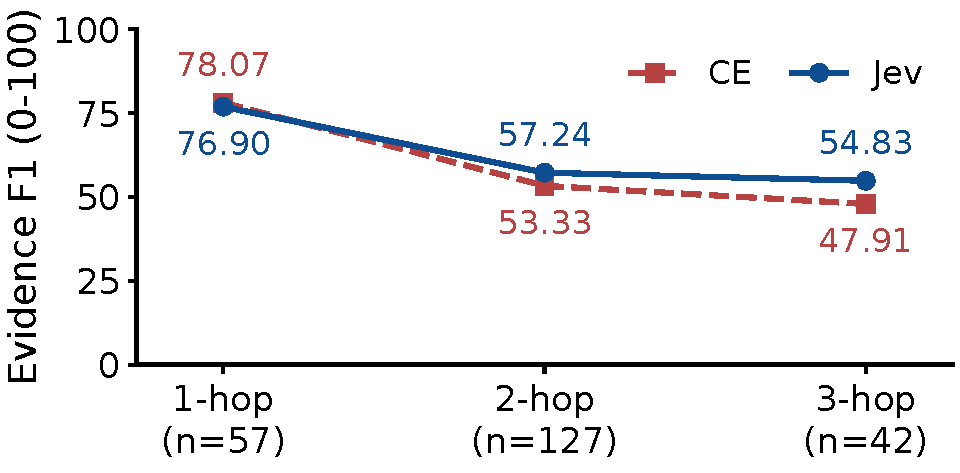
\includegraphics[width=\linewidth]{research/chapter4/figures/hop_f1.pdf}
    \caption{공식 hop별 최종 근거 F1. 표본 수는 각각 57, 127, 42문항이다.
    점은 기술통계이며 층별 신뢰구간은 산출하지 않았다.}
    \label{fig:ch4_hop_f1}
\end{figure}

3-hop의 평균 F1이 높아져도 완전 회수는 두 조건 모두
1문항(1/42, 2.38\%)에 머물렀다. 평균 F1의 증가가 모든 정답 근거의
확보로 이어지지는 않았다.

매핑 상태에 따른 성능 차이도 컸다. 전역 고유 gold 386개 중 27개가
corpus와 정확히 매핑되지 않아 29문항에 영향을 주었다.
완전 매핑된 197문항의 F1은 수정 CE 64.12점, Jev 67.21점이었으며,
영향을 받은 29문항에서는 각각 20.80점과 24.71점이었다.
두 집단에서 Jev의 점추정이 높았으나, 문자열 일치 점수는 gold 외
근거의 법률적 타당성까지 평가하지는 못한다. 이 진단은 29문항을
포함한 전체 분석을 보완한다.

문항별 F1은 대부분 같았고, 차이가 난 문항에서는 개선과 악화가
함께 관찰되었다. 반올림 전 차이에 $10^{-12}$의 동률 허용오차를
적용했을 때, Jev가 높은 문항은 32개, 같은 문항은 177개,
수정 CE가 높은 문항은 17개였다. 평균 개선은 이처럼 일부 문항의
변화에서 발생했다. 이 개수는 sourceㆍgold를 공유하는 문항들의
대응 결과를 기술하며, 독립 시행의 성공률을 뜻하지 않는다.
